% !TeX spellcheck = en_US
\documentclass[11pt, fleqn]{article}
%\usepackage{siunitx}
\usepackage{texfiles/SpeedyGonzales}
\usepackage{texfiles/MediocreMike}
\title{Logbook for 02466}
\author{Oskar Eiler Wiese Christensen, s183917@student.dtu.dk \\ Anders Henriksen, s183904@student.dtu.dk}

\begin{document}
	\maketitle
	
\section*{Project Meetings}

\subsection*{Week 1: 5.2.20 - 11.2.20}
We had no project meeting this week, as our group had not yet been created.

\subsection*{Week 2: 12.2.20 - 18.2.20}
\textbf{Questions:} At this point, there have not been many questions, as we had not started work on the project. Some things we have not been able to find answers for, though, is who will carry out the examination and how long the report should be. \\
\textbf{Reading:} For the end of next week, we will attempt to read the central article to this project, "equality of opportunity in supervised learning", without necessarily going too much into the details. \\
\textbf{Implementation:} We will start implementing the neural network immediately, as this will be the foundation for the rest of the project. \\
\textbf{Decisions:} We have decided that we mainly want to work on the project together, and as such, most of the rest of the implementations or results will be contributed towards by the both of us. Dagh is stuck in China because of corona and will therefore not be coming to the meetings and will work from China.

\subsection*{Week 3: 19.2.20 - 25.2.20}
\textbf{Questions:} At this point in time, we do not have many questions for the meeting next week. \\
\textbf{Reading:} For the rest of this week, we read different articles online, in order to get a better understanding of how bias is defined and how there might be differences in how papers define bias. \\
\textbf{Implementation:} For the rest of this week, we continued implementing the neural network for classification on the dataset. Meanwhile, we will also attempt to implement bayesian optimization and random forest, as this will show how efficient the neural network can become. \\
\textbf{Results:} Before the next supervisor meeting, the research questions, project canvas, gantt chart ect. should be finished, as they need to be done by wednesday next week. \\
\textbf{Decisions:} We have made the decision that the network should not have a binary output but rather be made to use a threshold to distinguish the different classes.

\subsection*{Week 4: 26.2.20 - 3.3.20}
\textbf{Questions:} How is the data we were working with different than what we were supposed to be using? Is it a good idea to use multiple datasets or more classifiers? \\
\textbf{Reading:} For this week, we have been advised to read the articles online about how ProPublica have analyzed the COMPAS algorithm. \\
\textbf{Implementation:} In regards to implementation, the machine learning notebook has now been setup to run on different types of data (mostly because it seems that the wrong data was used to begin with). Normalization functions were also put in place to reduce the exploding gradient problem as much as possible. \\
\textbf{Decisions:} We have decided, as evident in the last section, to change the dataset we have been using so far, as this seems to be similar but not equal to the dataset we are actually supposed to train a model on. \\

\subsection*{Week 5: 4.3.20 - 10.3.20}
\textbf{Questions:} Should feature selection be a part of the methods section? How can permutation be used to show bias in the data and model? How can bias correction from "equality of opportunity" be implemented properly? \\ 
\textbf{Reading:} Not much reading will be necessary for this week. \\
\textbf{Implementation:} We will implement a dataprep function, as this will make the code more structured. Meanwhile, it would also be good to show the bias in the data using more plots, and random forest still has to be finished. \\
\textbf{Decisions:} We have decided to delete the classifier on the old dataset, as this will not be usable for any of the rest of the project. We have also determined that Dagh does not seem to reply to our messages, so we will let him contact us if he wants to be a part of the group, as being stuck in China due to coronavirus probably makes project writing difficult.

\subsection*{Week 6: 11.3.20 - 17.3.20}
\textbf{Questions:} What is lacking in our mid-way evaluation? Do we need to re-write something? Does anything seem to be finalized at this point in time? \\
\textbf{Reading:} There will not be much reading for this week except for some other scientific papers to write the state-of-the-art section. \\
\textbf{Implementation:} We hope to implement a baseline model, so it is possible to compare our neural network with something unbiased. \\
\textbf{Results:} For this week, we will put more focus into writing references, as we have not been focusing on this otherwise. We will also be writing the data, ethics and introduction elements for the mid-way evaluation. \\
\textbf{Decisions:} We have decided that most of this week should be focused on writing, while letting programming take a backseat for a little while.

\subsection*{Week 7: 18.3.20 - 24.3.20}
\textbf{Questions:} What is the other group's impression of the report? \\
\textbf{Reading:} We will keep on reading more about state-of-the-art and other methods, that might be useful to implement or mention at some point. \\
\textbf{Results:} This week, we mostly focus on correcting the stuff we have learned from the previous supervisor meeting as well as generelly writing more and correcting spelling mistakes. We will also write the "contributions" part of the report and write more about bias generally. We will also start working on providing feedback for the group that we are supposed to give feedback. \\
\textbf{Decisions:} We will also not be doing much implementation this week, as other parts of the project writing are more important at this point in time.

\subsection*{Week 8: 25.3.20 - 31.3.20}
\textbf{Questions:} By giving the network "race" as an input, are we giving it too much to work with? And will the bias be removed if we remove "race"? \\
\textbf{Reading:} Reading will generally focus on other ways to classify data. \\
\textbf{Implementation:} This week, we will attempt to make bayesian optimization work and will also try to make some ROC-curves. \\
\textbf{Decisions:} We have decided that we need to start implementing some of the bias-correction methods soon, as this will be an important part of the report in the end.

\subsection*{Week 9: 1.4.20 - 5.4.20}
\textbf{Questions:} Are the ROC-curves significantly different if the thresholds along the curve are not equal? Should we remove every race except for white and black people? We stil do not understand permutation test, so how does this work? Can permutation test be used at the same time as feature selection? \\
\textbf{Reading:} We will mostly be reading about ROC-curves and examining how it will be possible to properly implement them in our project. \\
\textbf{Implementation:} We will do everything in our power to make the two ROC-curves for white and black people look different, as similar ROC-curves mean that the races are not being treated in a biased manner. \\
\textbf{Decisions:} We have decided to focus much more on implementation for this next week. Meanwhile, we have also decided that Dagh is probably not going to contact us anytime soon, and as such, we will carry out the rest of the project ourselves.

\subsection*{Week 10: 15.4.20 - 21.4.20}
\textbf{Questions:} How are we supposed to understand section 3 of the paper? We also still do not understand how to implement permutation to test for bias. \\
\textbf{Reading:} We will read the "equality of opportunity" paper much more carefully and try to get as much information out of it as possible. \\
\textbf{Implementation:} For this week, we will be focusing on trying to check for bias for sex as well as race, and we will perform the first steps on the road to implement equal opportunity and equalized odds. \\
\textbf{Decisions:} We have decided to implement both equalized odds and equal opportunity, though at this point in time, we will not be implementing any other bias-correction methods.

\subsection*{Week 11: 22.4.20 - 28.4.20}
\textbf{Questions:} A large list of questions have been set up so we can ask Melanie and Sune these next week, in order to get a greater perspective on our project and the ethics of our project. \\
\textbf{Reading:} This week, we will be reading about permutation in order to implement this for our report and in our code. \\
\textbf{Implementation:} We will attempt to implement our understanding of permutation. We are also trying to fit the machine learning models to more data, as this might shed light on whether the ROC-curves have been implemented poorly.

\subsection*{Week 12: 29.4.20 - 5.5.20}
\textbf{Questions:} Are the points from equalized odds supposed to land directly on top of each other? What if they don't? Could the slight difference be due to estimations? \\
\textbf{Reading:} We will be spending a lot of time reading about the bias correction methods from the paper and we will also read the paper a few more times in order to fully understand their methods. \\
\textbf{Implementation:} We will make the matrix showing distributions of white and black people and we will try our best to implement equal opportunity and equalized odds. \\
\textbf{Decisions:} We are focusing only on the implementation of bias-correction methods this week, as there are not many weeks left and we have not made much progress in the sense that neither equal opportunity nor equalized odds work properly at this time.

\subsection*{Week 13: 6.5.20 - 12.5.20}
\textbf{Questions:} Is it necessarily wrong that the point is jumping a bit back and forth, if it is just a question of small estimation mistakes? \\
\textbf{Implementation:} We will finalize the implementation of equal opportunity and equalized odds. Meanwhile, we need to try to understand why the blue point in the plot from equalized odds is jumping around so much. \\
\textbf{Decisions:} We have decided that it might not be a good idea to try to get bayesian optimization to work, since we have had experience from the exam that it might take a while to implement and might not give that much of an increase in accuracy.

\subsection*{3-Week Period - Week 1: 4.6.20 - 10.6.20}
\textbf{Questions:} 
\textbf{Reading:} 
\textbf{Implementation:} 
\textbf{Decisions:} 

\subsection*{3-Week Period - Week 2: 11.6.20 - 17.6.20}
\textbf{Questions:} 
\textbf{Reading:} 
\textbf{Implementation:} 
\textbf{Decisions:} 

\subsection*{3-Week Period - Week 3: 18.6.20 - 24.6.20}
\textbf{Questions:} 
\textbf{Reading:} 
\textbf{Implementation:} 
\textbf{Decisions:} 


\section*{Supervisor Meetings}

\subsection*{Week 1: 5.2.20 - 11.2.20}
We had no supervisor meeting this week, as the project had not started yet.

\subsection*{Week 2: 12.2.20 - 18.2.20}
In this meeting, we set the foundation for how the following supervisor meetings will proceed. Our meeting will be at 13:00 every wednesday and the other group that has the same topic will have their meeting at 14:00. Every second week for the first part of the project process, our meetings will be combined, so we can learn from each other's mistakes and get common issues sorted out. \\
We will start the work on the research questions after this meeting and will be focusing on questions with concrete success criteria and a clearly defined scope. We were also urged to consider implementing multiple classification and bias correction algorithms. For next week, we will have outlined some research questions to go through.

\subsection*{Week 3: 19.2.20 - 25.2.20}
During this week's meeting, we mostly considered which way the project could go and how we would like to proceed in the following weeks. Since the original analysis of the data was made using simple logistic regression, we came to the agreement that it would be interesting to apply a deeper model to the data, which also fits the implementation of the neural network. We also realized that causality between the different variables might be a relevant subject to touch upon. Regarding the data, we need to consider that a biased dataset might just show that black people actually perform more crime that white people, so the ML-model might not even be truly biased. Rather, it just finds the true distribution of crime in the population. Lastly, we should not be too ambitious when writing the research question, as they should all be answered by the end of the project writing process.

\subsection*{Week 4: 26.2.20 - 3.3.20}
This week, the supervisor meeting was short, as there was not many questions to be answered. The meeting generally revolved around bias. In order to show the existence of bias in the data, permutation of the data could be used to show whether there is actually bias in the data. It is also not possible to use other methods than figures to find bias in the data, as a model needs to be trained on the data in order to show the inherent bias. Lastly, a ground truth needs to be set up, such that it can be proven whether there is actually a bias in the data.

\subsection*{Week 5: 4.3.20 - 10.3.20}
As the mid-way evaluation has to be ready before within a few weeks, we have decided with our supervisor that we will have this ready early, so she will be able to take a look at it and see if the report is on the right track so far. \\
It could still be a good idea to make a baseline such as a model that guesses only on the biggest class or something like logistic regression. Meanwhile, we still have to implement actual predictions on the random forest classifier. Futhermore, more plots could be constructed to show bias in the data and we still have to show statistical significance.

\subsection*{Week 6: 11.3.20 - 17.3.20}
There were many questions from the previous week, so most of the meeting was spent going though these. Feature selection is an important part of the report and should be prioritized, as this allows for a way to show where the bias in the data could be coming from. It would also be a good idea to make a table of every variable in the dataset, as this seems to never have been done before. To implement equality of opportunity bias correction methods, the convex hull should be considered. Regarding bias and how to implement the methods, it could also be an idea to follow ProPublica's analysis closely. As a last point for this meeting, we decided to make a Slack for all of us, as DTU might close soon due to coronavirus.

\subsection*{Week 7: 18.3.20 - 24.3.20}
For this supervisor meeting, our supervisor gave feedback for our mid-way evaluation deliverable. For this, we have been told to put more focus on the fact that a table of variables has never been made before. Bias is also a result and should thus not be a part of the methods section. We noted that neural network model has suddenly stopped working, and out supervisor mentioned that it might be worth it to try to create synthetic data in order to make the model learn again. Generally for the report, it is important to hold the hand of the reader a lot more. It is also important to stress that only 1-2 bias correction methods should be implemented, as we have used pluralis for every mention of this. There are other kinds of bias, so these could also be looking into to get some more meat on the bones of the methods section.

\subsection*{Week 8: 25.3.20 - 31.3.20}
We did not have a supervisor meeting this week, but we did meet with our feedback group, so this meeting slot will be dedicated to the notes from this meeting. Generally, they are very positively surprised by the table of variables and the entire introduction. They find the plots and illustrations confusing, because low and medium have been interchanged. Instead of just using the plots to show bias in the data, we should also use something like a matrix, which shows the actual distribution better. The other races should also be removed from the plots. For the methods, they found that bayesian optimization takes up way to much space compared to how little it should mean in the grand scheme of our report. Bias is not defined well at all and needs to be much more clearly defined. Lastly, we need to show why we only decide to use 9 of the 50 features in the dataset.

\subsection*{Week 9: 1.4.20 - 5.4.20}
The two ROC-curves from the different races seem to be way to similar, so we need to figure out why they are so close to each other.If we are not able to make the ROC-curves look significantly different from each other, it might be necessary to try to find an implementation online. Race needs to be a part of the dataset, since it is important the the network can actually find the biased variable. The rest of the meeting will only be focussing on variables that we have not yet found the meaning of. c\_days\_from\_compas is the difference between compas\_screening\_date and c\_offence\_date. c\_offence\_date is a replacement variable for when it is not possible to determine the actual date of the offence.

\subsection*{Week 10: 15.4.20 - 21.4.20}
We had many questions for this meeting too, so a lot of the time will be spent on these. The other races might be a kind of outlier in the data, so it could be a really good idea to remove them from the dataset. To show that the model is truly biased using permutation tests, a bunch of tests are performed showing how the model will perform if there is no correlation between any of the variables. If our model does better than this, then our model is significantly better than average but might also be biased. Since the ROC-curves are very close to each other, it might be a good idea to talk about this in the discussion. It might be an idea to check if race is as biased in the dataset as race. It is luckily possible to implement both equal opportunity and equalized odds, since the thresholds seem to make most of the difference in results.

\subsection*{Week 11: 22.4.20 - 28.4.20}
We did not have much to talk about for this meeting, as we had a lot of stuff to do. As such, we had a very short meeting. Permutation cannot directly show bias, so what we have done using permutation is already fine. For the rest of the meeting, we showed that we have fittet the neural network to a completely new dataset and we had a walk-through of section 3 of the report.

\subsection*{Week 12: 29.4.20 - 5.5.20}
Meeting with Melanie:

DATA AND DATA PREPARATION
How do we show with illustrations that there could be bias in the data?
She herself has found TP, TPR, FP, FPR for both classes. We can also normalize the plots.


Do we need to do class balancing to get the right result?
In practice, the classes are never equal. This can be taken into account in the loss function.

THE BINARY NEURAL NETWORK
You might need to do standard deviation or cross validation so you can see the error of accuracy.
The same can be implemented with multiple test sets.
Do permutation, then the result should be the same accuracy as for a baseline.

COMPARISON TO BASELINE
How to compare a classifier? Do you use a baseline or can you really compare to something like real judges?
We only need to run the test through baseline.


BIAS CORRECTION METHOD
How is it decided if FP or TP is the most important priority?
It depends on the application.
Sensitivity in medicine shows that it depends on the application.


Meeting with Sune:

Where does the bias come from?
We can investigate that because you could think that it comes from the algorithm. In principle, bias comes from an inequality between two groups. Inequality must be "unfair" to be bias.

Investigate: Does a fair process guarantee a fair outcome?

If you want to make a good classifier, you can include the things that give a good result. It also depends on the context, because sometimes sensitive data is not needed.
There must be a logical connection between what one uses and what one has to decide.


You must avoid data being stolen, but there are rules to follow.

Are facebook and snapchat not be responsible for when data is leaked?
It is really easy to get data from public social media. So it is also their responsibility.

How to avoid bias in humans?
It can be avoided with education and habit, because it is somehow built into our nature.

We use algorithms to gain a better understanding of our own way of thinking.

Are there problems in the way we define bias?
We must talk about that another time, it is a very complex discussion.

\subsection*{Week 13: 6.5.20 - 12.5.20}
Since the exams are well on their way, we will not be having supervisor meetings untill the first week of the 3-week period. There will also not be much work on the project itself, as the exams have the priority. We have also determined that it could be good practice for us to to present our work for Sune some time before the exam, as this would also help him to better understand the topics used in the project. \\
The blue dot that is supposed to be on top of the green dot seems to jump around sometimes, which might not be correct, so we should look though the code to try to spot mistakes. It could also be a good idea to finish implementing equal opportunity. \\
For future work, it could be interesting to take a look at pre-processing bias-correction methods (bias-correction used before the network has been trained), though this is only necessary if there is time to implement it. As a point in the discussion, it could be an idea to talk about the accuracy-fairness trade-off, since this will probably be an important dilemma in the years to come.

\subsection*{3-Week Period - Week 1: 4.6.20 - 10.6.20}


\subsection*{3-Week Period - Week 2: 11.6.20 - 17.6.20}


\subsection*{3-Week Period - Week 3: 18.6.20 - 24.6.20}


		
\newpage
\newpage
\section*{Project Meetings}
	
	%Questions \\
	%Reading, who and what \\
	%Implementation, who and what \\
	%Results, who and what \\
	%Decisions, who and what, what do you do alone, what do you do together
	
	\textbf{Week 08:}  19.02.2020 \\\\
	\noindent
	Hvilke bias eksisterer i dataen? \\ 
	\begin{figure}[H]
		\centering
		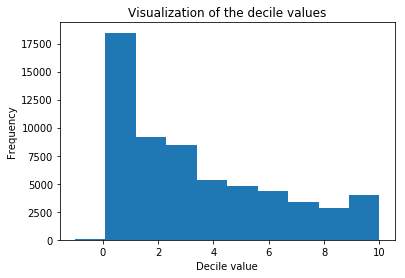
\includegraphics[width=0.3\linewidth]{billeder/decil.png}
	\end{figure}

	\begin{figure}[H]
		\centering
		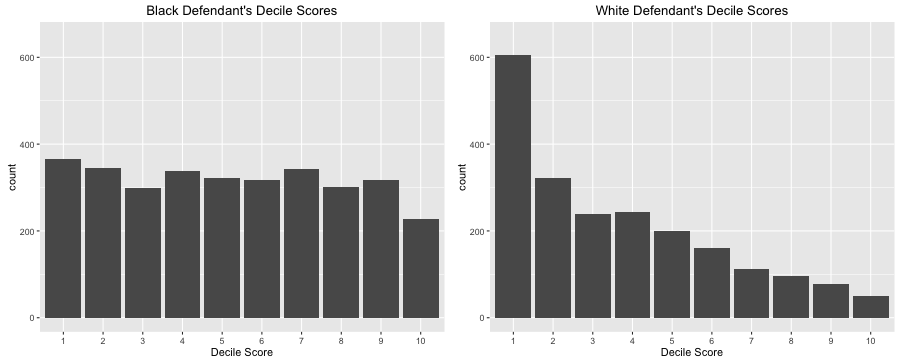
\includegraphics[width=0.7\linewidth]{billeder/black_white}
	\end{figure}
	\noindent
	There exists a recial bias in the dataset, which is indicated by the histograms above. 
	\\\\
	\textbf{Week 10:}  03.03.2020 \\\\
	\noindent
	Spørgsmål til næste møde: \\
	Hvordan skal dataen permuteres ? (Kun indenfor en kategorisk variabel eller hele datasættet) \newline 
	Kan man se bias ud fra confusion matrix?? \\ 
	Skal man vise, at der en statistisk forskel på de to confusion matricer? \\ \\
	\textbf{Noter} \\ 
	Lav nogle flere plots for at vise, om der er bias i selve data. Undersøg, hvor mange der får 1 i recidivism både af sorte og hvide.
	\newline
	Det ville være smart at finde noget statistisk signifikans. Man kan finde en p-værdi ved at bruge permutationstests.
	\newline
	Lav predictions med random forests.
	\newline
	Equal opportunity er godt resultatet, som vi ser fra vores data. Man kunne plotte equal opportunity som netværket bliver trænet.
	\newline
	Lav en slags baseline som logistisk regression for at se, om de begge er biased eller om de klarer sig lige godt.
	\newline
	Vi skal senest have midvejafleveringen klar d. 16, så Aasa kan læse det igennem.	
	\\\\	
	\textbf{Week 11:}  10.03.2020 \\\\
	\noindent
	Spørgsmål:
	\begin{itemize}
		\item  Hvordan skal vi lave feature selection for at se om de forskellige attributes påvirker modellen? Skal det stå som et afsnit i metoder?
		
		\item 4454, i forhold til at tage udgangspunkt i dataen, hvordan kan bias påvises vha. permutationstest. 
		
		\item Hvordan man helt præcist skal implementere Hardt et al. (post hoc correction)
		
		\item Hvordan skal vi finde bias i datasættet? 
		
		\item domain adaptation / transfer learning
		
		\item ting fra ICML / ECML , ICLR, Fair 
		
	\end{itemize}
	
	Skrive om feature selection i metode
	
	
\section*{Supervisor Meetings}
	
	\textbf{Week 07:}  12.02.2020 \\\\
	\noindent
%	Presentation of results since last meeting \\
	Meeting notes: \\ Fællesmøder samt personlige møde. (Hver anden uge er individuele). \\0. Vi får et datasæt (COMPASS) - ligger online \\
	1. Hvordan er dataen skæv? (Hvilke bias eksisterer i dataen) (Hvordan finder man helt præcist ud af det?) (Hvad betyder det at der er en bias?) \\
	2. Hvad gør skæv data ved min algoritme? (hvad betyder bias i en algoritme) (Hvordan kvantificeres/verificeres bias i algorimten?) \\
	3. Equality of Opportunity in Supervised Learning (forstå, implementer og valider) \\ 
	4. Etisk diskussion (Sune Filosof)
	\\\\\\\\
	\textbf{Week 08:}  19.02.2020 \\\\
	\noindent
	%	Presentation of results since last meeting \\
	Meeting notes: \\ Feature extraction
	\\\\
	Action points for next week: N/A
	\\\\\\\\
	\textbf{Week 09:}  26.02.2020 \\\\
	\noindent
	%	Presentation of results since last meeting \\
	Meeting notes: 
	\\\\
	Action points for next week
	\begin{itemize}
		\item  
	\end{itemize} 
		
	
\end{document}
